\documentclass[tikz,border=12pt]{standalone}
\usepackage[T1]{fontenc}
\usepackage{lmodern}
\usepackage{tikz}
\usetikzlibrary{arrows.meta,positioning}

\definecolor{navy}{HTML}{0C171F}
\definecolor{green}{HTML}{00F700}

\tikzset{
  component/.style={
    draw=navy,
    line width=1.2pt,
    rounded corners=5pt,
    minimum width=5.3cm,
    minimum height=2.65cm,
    text width=4.8cm,
    align=center,
    text=navy,
    fill=none,
    font=\fontsize{11}{13.5}\selectfont
  },
  reward/.style={
    component,
    minimum width=5.6cm,
    text width=5.1cm
  },
  flow/.style={
    -{Latex[length=3.4mm,width=2.2mm,fill=green]},
    draw=navy,
    line width=1.4pt
  },
  operator/.style={
    text=green,
    font=\bfseries\fontsize{22}{24}\selectfont
  }
}

\begin{document}
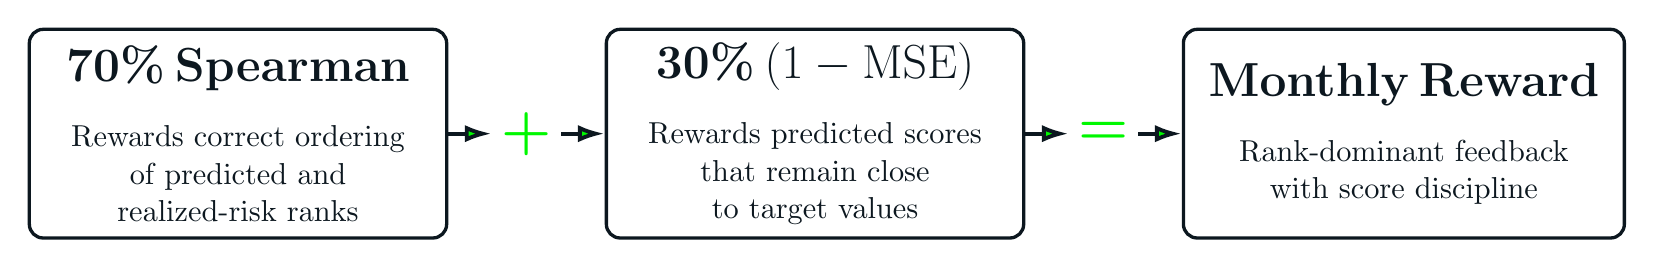
\begin{tikzpicture}
  \node[component] (spearman)
    {\textbf{\fontsize{16}{19}\selectfont 70\% Spearman}\\[10pt]
     Rewards correct ordering\\of predicted and realized-risk ranks};

  \node[operator, right=0.55cm of spearman] (plus) {+};

  \node[component, right=0.55cm of plus] (mse)
    {\textbf{\fontsize{16}{19}\selectfont 30\% \(\left(1-\mathrm{MSE}\right)\)}\\[10pt]
     Rewards predicted scores\\that remain close to target values};

  \node[operator, right=0.55cm of mse] (equals) {=};

  \node[reward, right=0.55cm of equals] (reward)
    {\textbf{\fontsize{16}{19}\selectfont Monthly Reward}\\[10pt]
     Rank-dominant feedback\\with score discipline};

  \draw[flow] (spearman.east) -- (plus.west);
  \draw[flow] (plus.east) -- (mse.west);
  \draw[flow] (mse.east) -- (equals.west);
  \draw[flow] (equals.east) -- (reward.west);
\end{tikzpicture}
\end{document}
